\section{Contributions to the mass resolution for $\chicone \rightarrow J/\psi \mu^+ \mu^-$}
\label{sec:chic}
%
The $\chicone \rightarrow J/\psi \mu^+ \mu^-$ invariant mass is
calculated using a kinematic fit \cite{Hulsbergen:2005pu} with constraints applied on the
$J/\psi$ mass and the pointing of the candidate to the primary
vertex (PV). Consequently,  the mass resolution can be factorized into three components: the
momentum resolution for the muons from the virtual photon, the muon
track slopes and the parameters of the $J/\psi$. From the previous
studies of this mode in Ref.~\cite{Anderlini:2270922} the resolution is known to $\sim 1.7
\mevcc$. This is confirmed in Fig. \ref{fig:gcb} where the mass
distribution for selected candidates is plotted together with a fit to
the sum of a Crystal Ball \cite{Skwarnicki:1986xj} plus a Gaussian function is superimposed. The
resolution returned by the fit, defined as $\sqrt{ f \cdot \sigma_1^2
  + (1-f) \sigma_2^2}$, is $1.7 \mevcc$.   
\begin{figure}[htb!]
%\vspace{-5mm}
\begin{center}
\resizebox{3.5in}{!}{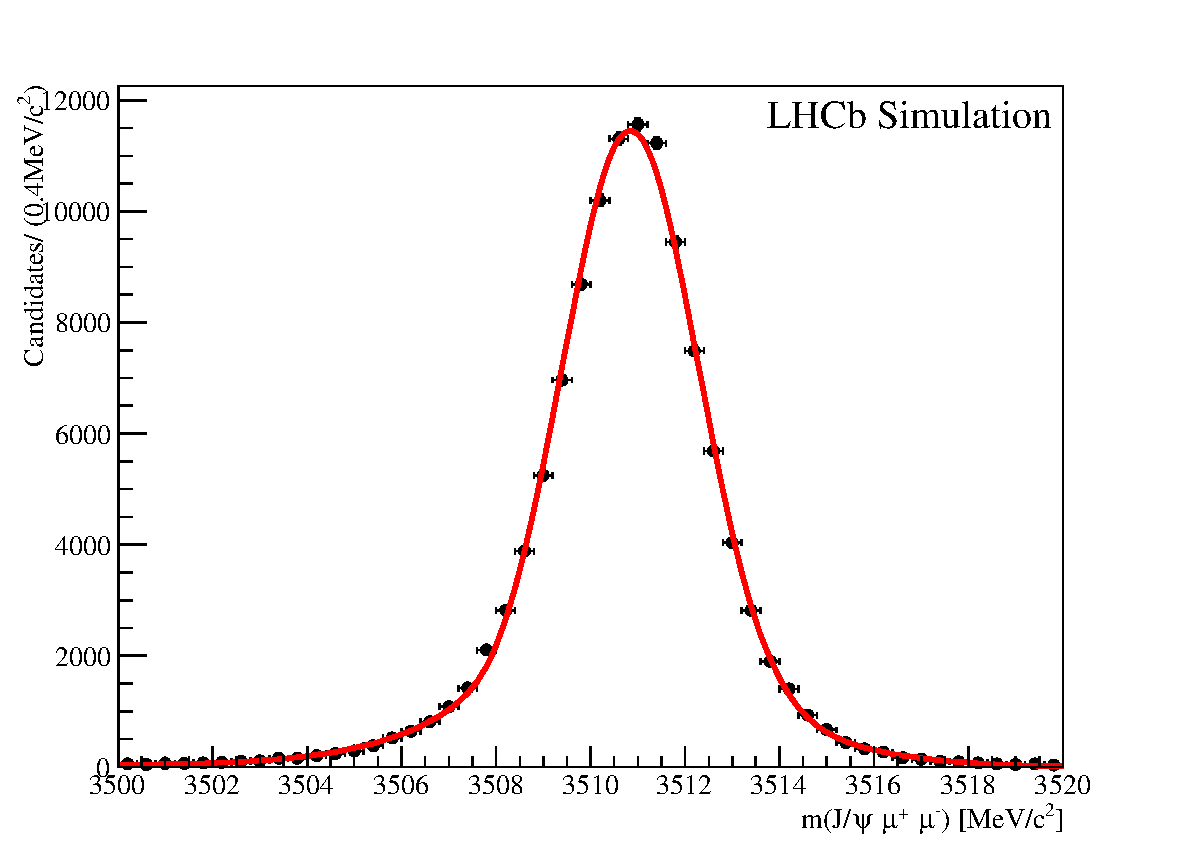
\includegraphics{figs/chic_1_GCB.pdf}}
%\vspace{-5mm}
\caption{\small  $J/\psi \mu^+ \mu^-$ invariant mass for the selected
  and truth matched $\chicone$ candidates in the simulation. }
\label{fig:gcb}
\end{center}
\end{figure}

To understand the relative importance of these contributions the
invariant mass is built using the Monte Carlo truth information together with  the
reconstructed momenta (slopes) of the
muons from the virtual photon and repeating the mass fit. The results
of this study are summarized in Table \ref{tab:rescontrib}. For this
decay mode, due to the low energy release, the most
important factor is the resolution on the track slopes. The contribution from the parameters of the mass constrained
particle, in this case the $J/\psi$, is small.
%
\begin{table}[htb!]
\caption{\small Contributions to the mass resolution for the $\chicone
  \rightarrow J/\psi  \mu^+ \mu^- $ decay mode. Reconstructed $p$
  the true slopes but reconstructed $p$ is used for the muon pair from
  the virtual photon. Reconstructed $tx,ty$ means the true $p$ but reconstructed $tx,ty$ is used for the muon pair from
  the virtual photon.  }
\begin{center}
\small
\begin{tabular}{l|c}
Condition & $\sigma [\mevcc]$   \\
\hline
Truth + Reconstructed $p$ & 0.9  \\
Truth + Reconstructed $tx,ty$ & 1.2\\
Truth + Reconstructed $p$ +Reconstructed $tx,ty$ & 1.6 \\  
Fully reconstructed & 1.7 \\
\end{tabular}
\end{center}
\label{tab:rescontrib}
\end{table}

The importance of the PV constraint in improving the resolution on the
track slopes can be seen in Fig. \ref{fig:sloperes}:  the application of the PV constraint improves the slope
resolution by a factor of two and
hence will improve the mass resolution considerably \footnote{Qualitiatively this
  makes sense: adding the PV information provides a high precision
  measurement of the track position at its origin point and allowing
  to correct for any multiple scattering in the RF foil.}. This explains why the standard
release of  \textbf{RapidSim} which uses the unconstrained slope resolution
overestimates the mass resolution for these decays.
\begin{figure}[h!]
\centering
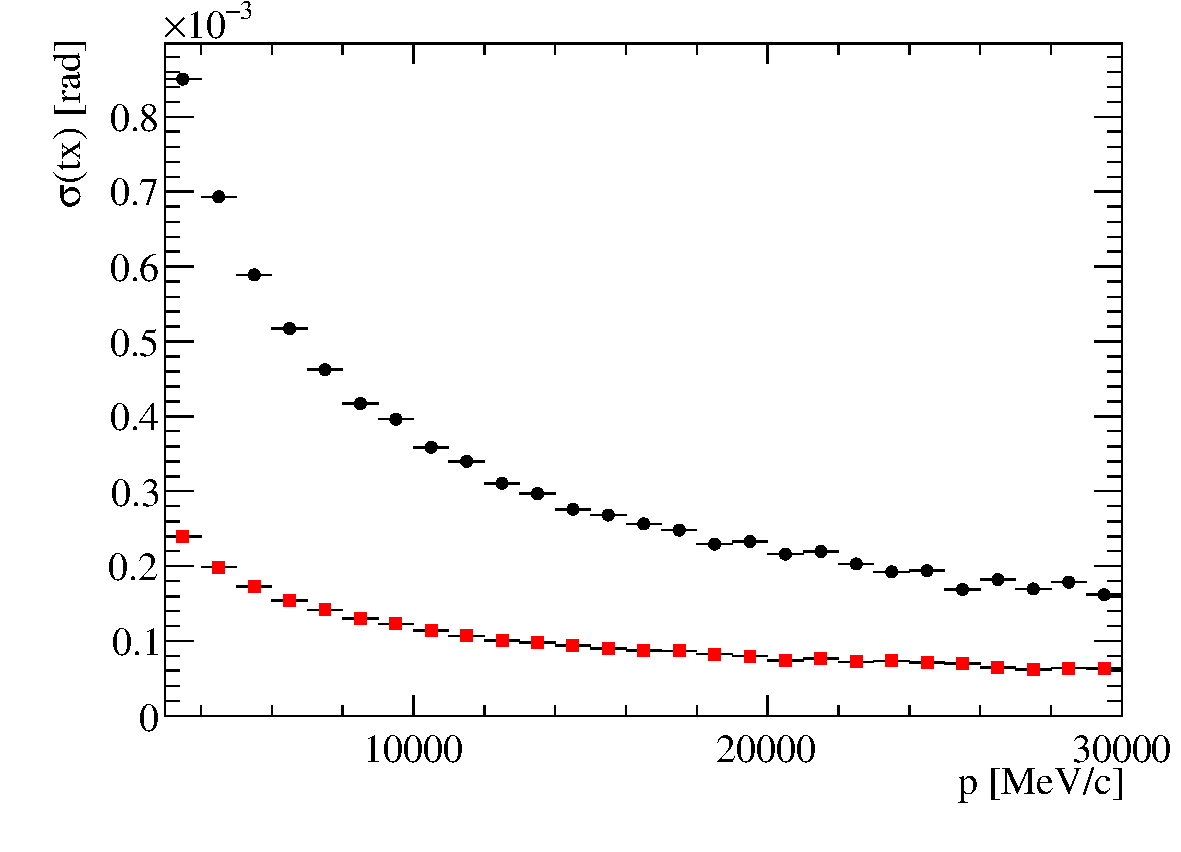
\includegraphics[width=0.48\textwidth]{figs/txres.pdf}
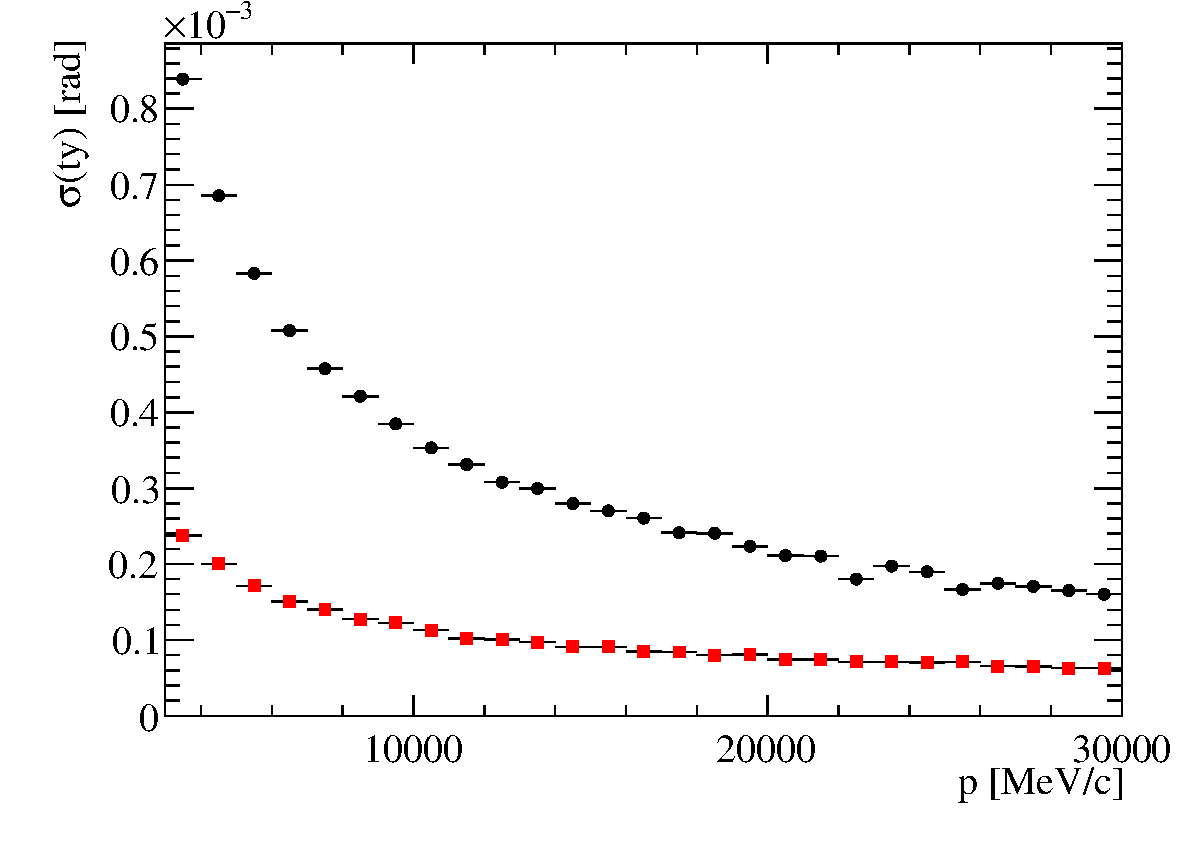
\includegraphics[width=0.48\textwidth]{figs/tyres.pdf}
\caption{(Left) Resolution on $tx$ versus $p$ before (black points) and after (red
  squares) the PV constraint is applied. (Right) Resolution on $ty$
  versus $p$ before (black points) and after (red
  squares) the PV constraint is applied for the muons from the virtual
  photon. In both cases the values are
  obtained by fitting a Gaussian to slices in $p$ to a 2-dimensional histogram.
   }
\label{fig:sloperes}
\end{figure}

To emulate the mass resolution the four-vectors of the muons and
$J/\psi$ are individually smeared, ignoring correlations. The parameterizations used for this
smearing are described in Section~\ref{sec:ep} - \ref{sec:res} and
takes into account the dependence of resolution on the particle kinematics. It will be
seen that this procedure reproduces the full simulation results well.